\section{Análisis de performance}
\subsection{Aclaraciones}
Para generar los siguientes análisis de performance, se creó un programa en \textit{Python} para generar una serie de problemas a computar, con y sin solución, desde $10$ hasta $n$ elementos. Se pueden describir los problemas como elementos de una matriz $Problema \ problemas[n][r]$ donde $Problema$ es una tupla del tipo $(T, values)$, $n$ es la cantidad máxima de elementos a evaluar y $r$ es la cantidad de repeticiones para cada problema de tamaño $n$. Es decir, la cantidad de veces que se va a repetir un experimento de $n$ elementos con el objetivo de mejorar las mediciones obtenidas. Es necesario aclarar que para toda repetición de un problema dado un $n$, sus valores $T$ serán iguales. Esto es necesario para poder estimar confiablemente la equivalencia de un cómputo $\mathcal{O}(1)$ en segundos. Esto se realiza dividiendo el valor de $T$ contra la cantidad de recursiones que demandó cada problema. De esta manera, se obtiene una cota $\mathcal{O}(n*T)$ aproximada en los análisis de programación dinámica.

\vskip 8pt

Además, cada problema es generado aleatoriamente con un $T$ entre $(999, 99999999)$. La mitad de los problemas tienen garantizada una solución. La otra mitad, no. La disposición de los elementos de los valores de $values$ con solución son equiprobables. Es decir, tienen los elementos que forman parte de la solución pueden estar en cualquier lugar de la lista. Es por eso que en algunos gráficos se podrá observar que ciertos problemas de $n$ elementos hayan sido solucionados más rápidamente que otros problemas de $k$ elementos, con $n > k$. Estos casos intentan ser apaciguados mediante la elevada repetición de los problemas para cada cardinal y luego a través de la "poda" del $5\%–10\%$ de las soluciones más rápidas para cada tamaño de problema. Es importante aclarar que todos los algoritmos resuelven exactamente los mismos problemas, asegurando justicia e integridad en las comparaciones.

\vskip 8pt

Específicamente, los experimentos fueron computados para $n = 10 ... 34$ con $r = 40$. Es decir, cada $n$ fue calculado 40 veces con el mismo $T$ pero distintas listas de valores de $n$ elementos.

\subsection{Fuerza Bruta}
\begin{figure}[H]
	\centering
	\begin{minipage}{0.48\textwidth}
		\centering
		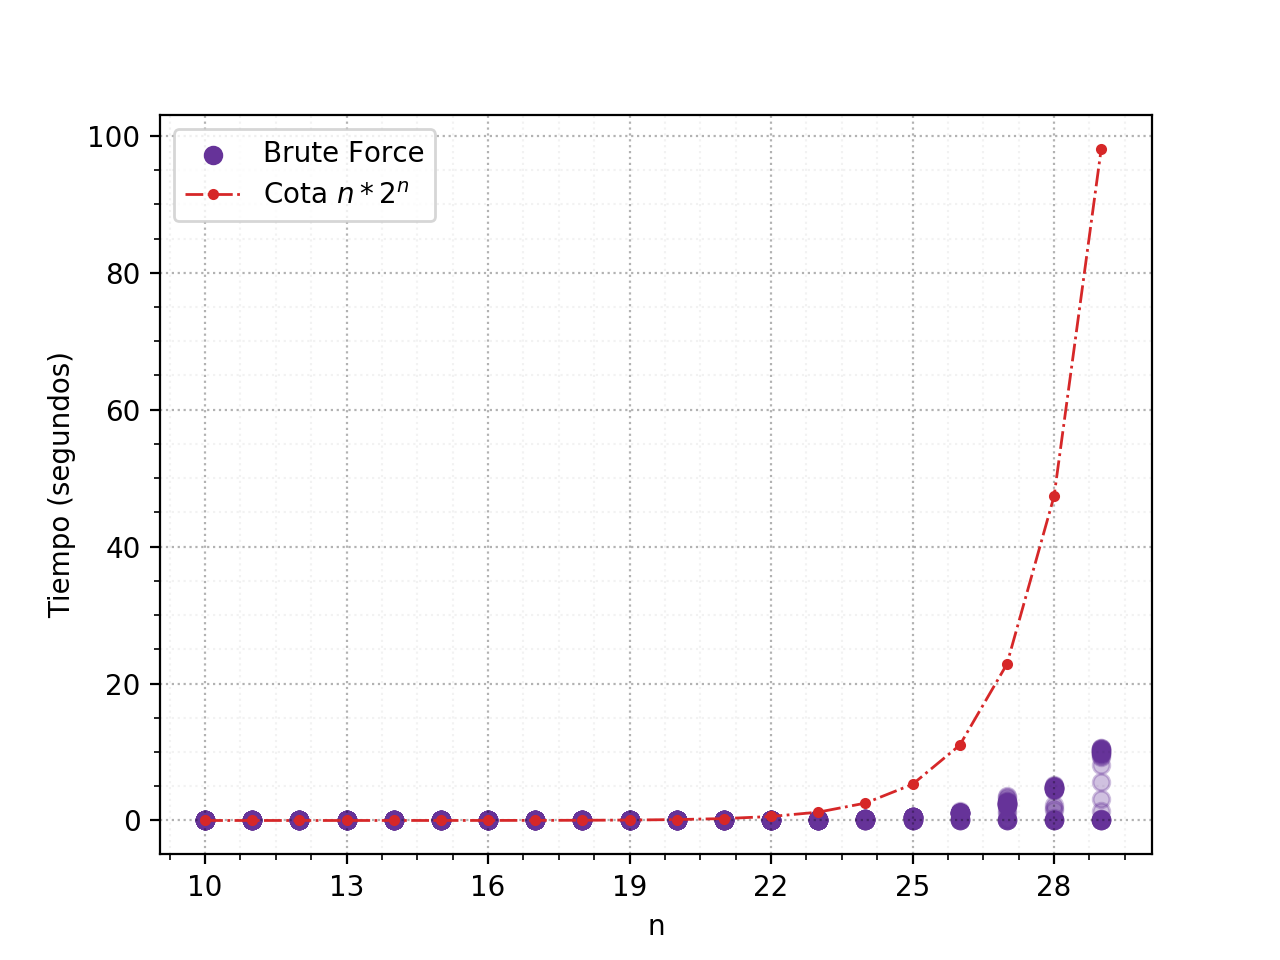
\includegraphics[width=1\textwidth]{bf-and-cota}
		\caption{\footnotesize Segundos consumidos (en escala lineal) en función de la cantidad de elementos de $values$.}
		\label{fig:plot-bf-and-cota}
	\end{minipage}%
	\hspace{0.03\textwidth}
	\begin{minipage}{0.48\textwidth}
		\centering
		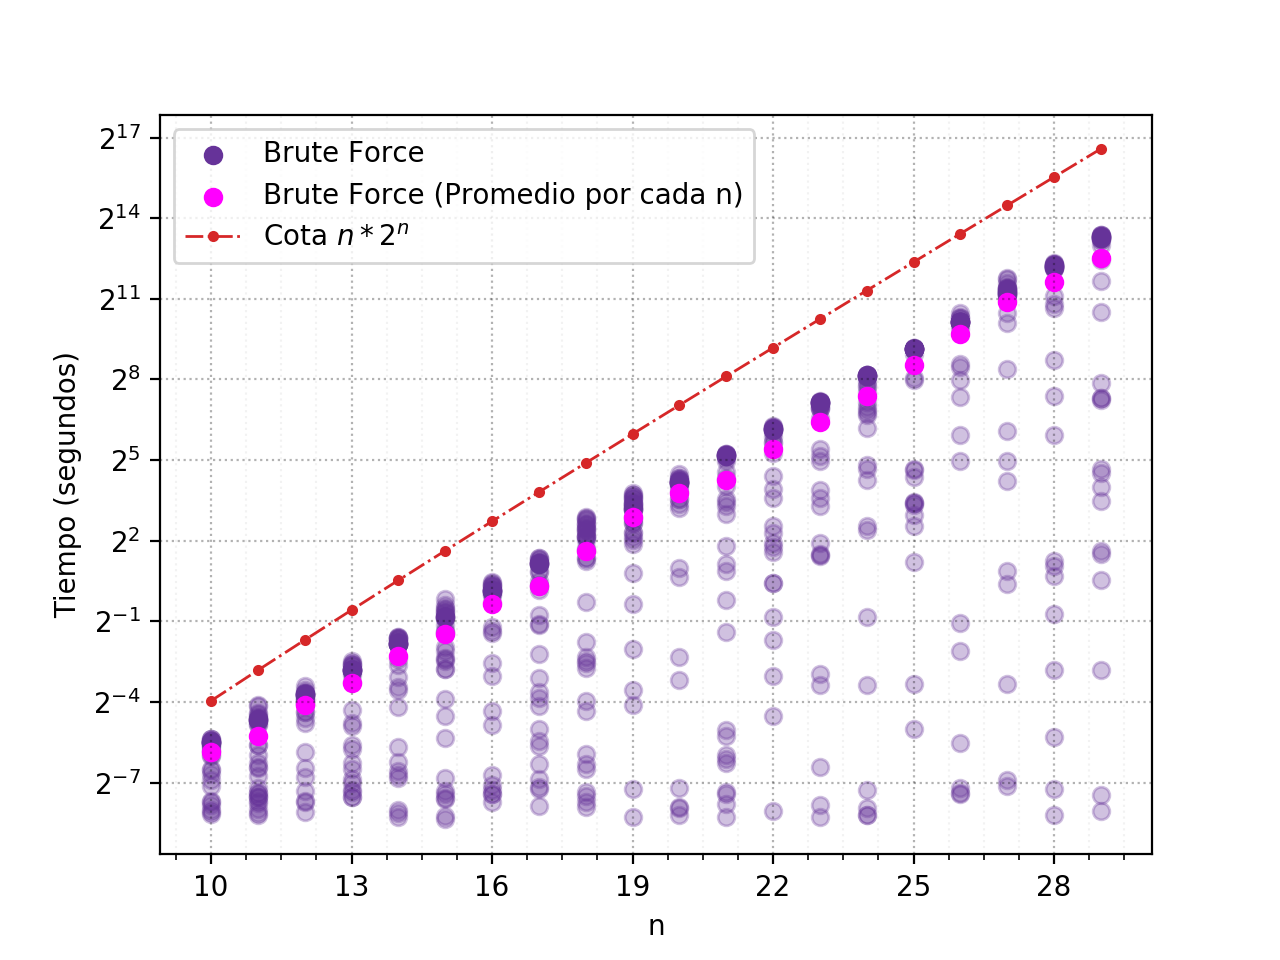
\includegraphics[width=1\textwidth]{bf-and-cota-log}
		\caption{\footnotesize Segundos consumidos (en escala logarítmica) en función de la cantidad de elementos de $values$.}
		\label{fig:plot-bf-and-cota-log}
	\end{minipage}%
\end{figure}

En estos gráficos se puede observar – en púrpura – todas las computaciones para cada problema de cardinal $n$. Mientras que, en rojo, se puede apreciar la cota teórica del algoritmo de fuerza bruta. Ambos experimentos apoyan empíricamente la hipótesis "\textit{El algoritmo de fuerza bruta tiene complejidad} $\mathcal{O}(n*2^n)$". Además, queda claro el comportamiento exponencial de la solución. Esta hipótesis puede ser reforzada con el siguiente experimento:

\begin{figure}[H]
	\centering
	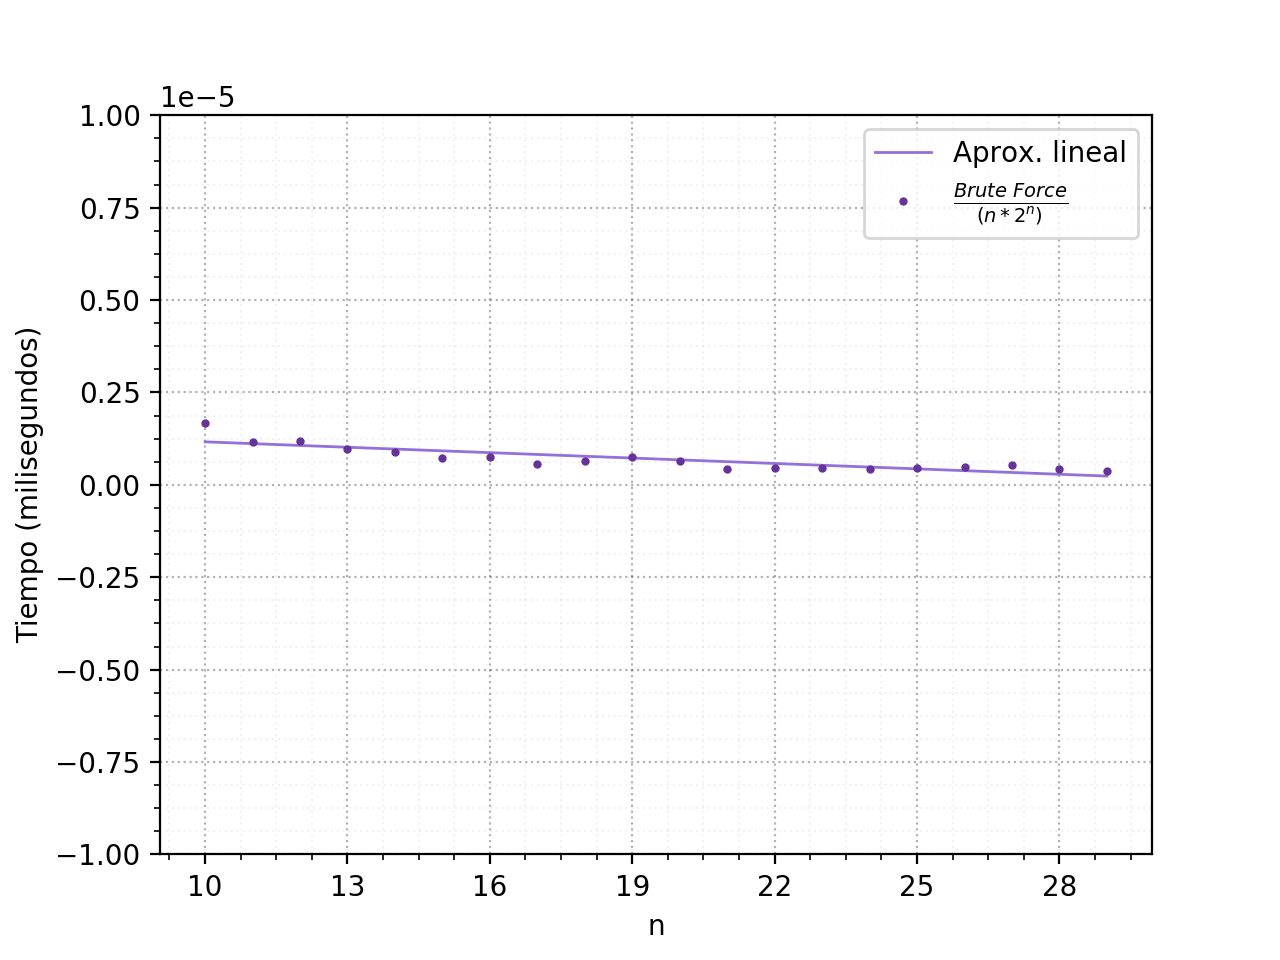
\includegraphics[width=0.5\textwidth]{bf-div-cota}
	\caption{\footnotesize Segundos consumidos en función de la cantidad de elementos de $values$ dividido $n*2^n$}
	\label{fig:plot-bf-div-cota}
\end{figure}

De esta manera, queda explicitada la tendencia de la complejidad del algoritmo con respecto a su complejidad: siempre será ampliamente menor.

\subsection{Back Tracking}
\begin{figure}[H]
	\centering
	\begin{minipage}{0.48\textwidth}
		\centering
		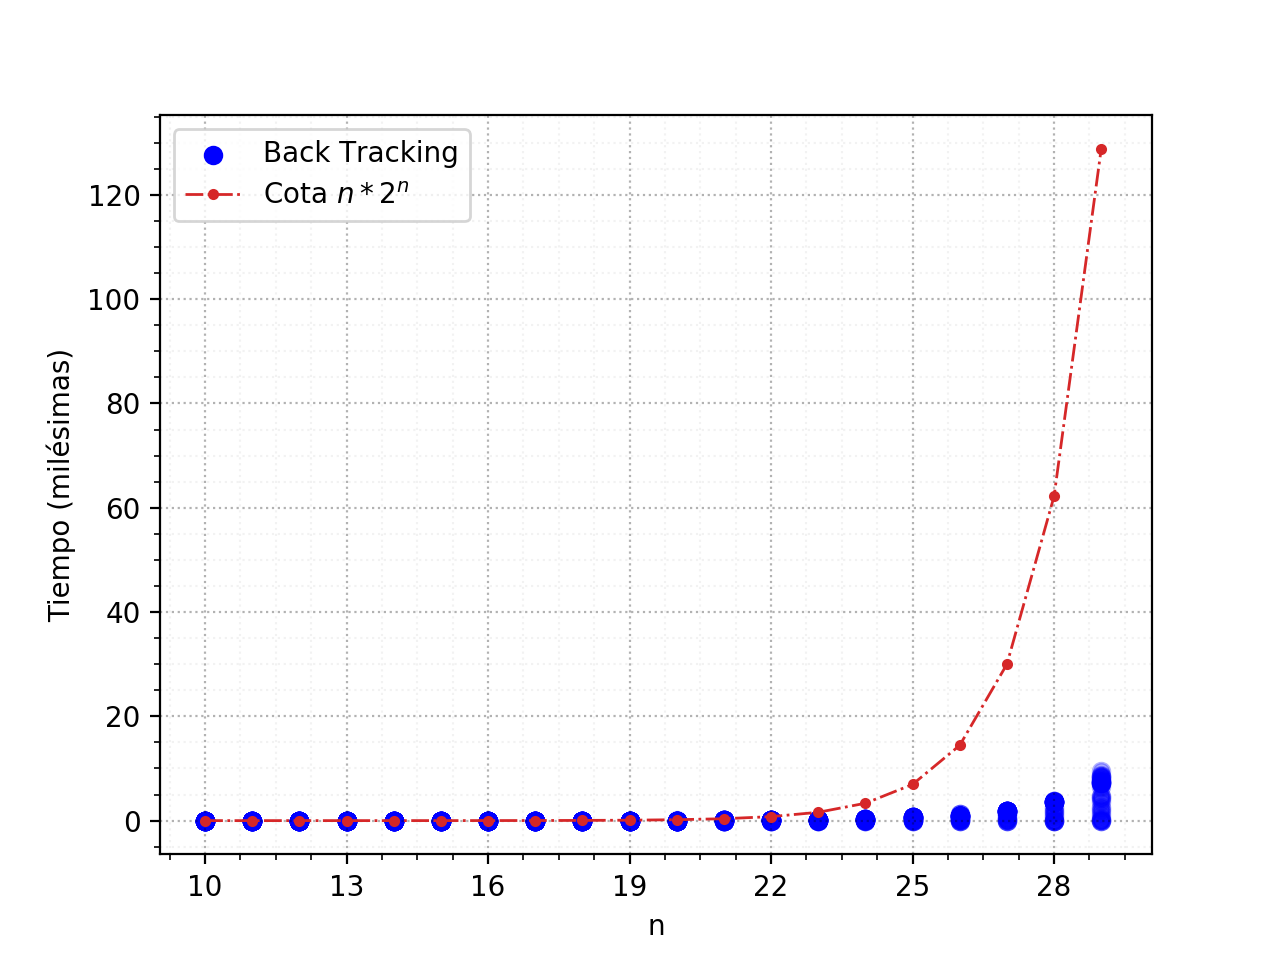
\includegraphics[width=1\textwidth]{bt-and-cota}
		\caption{\footnotesize Segundos consumidos (en escala lineal) en función de la cantidad de elementos de $values$.}
		\label{fig:plot-bt-and-cota}
	\end{minipage}%
	\hspace{0.03\textwidth}
	\begin{minipage}{0.48\textwidth}
		\centering
		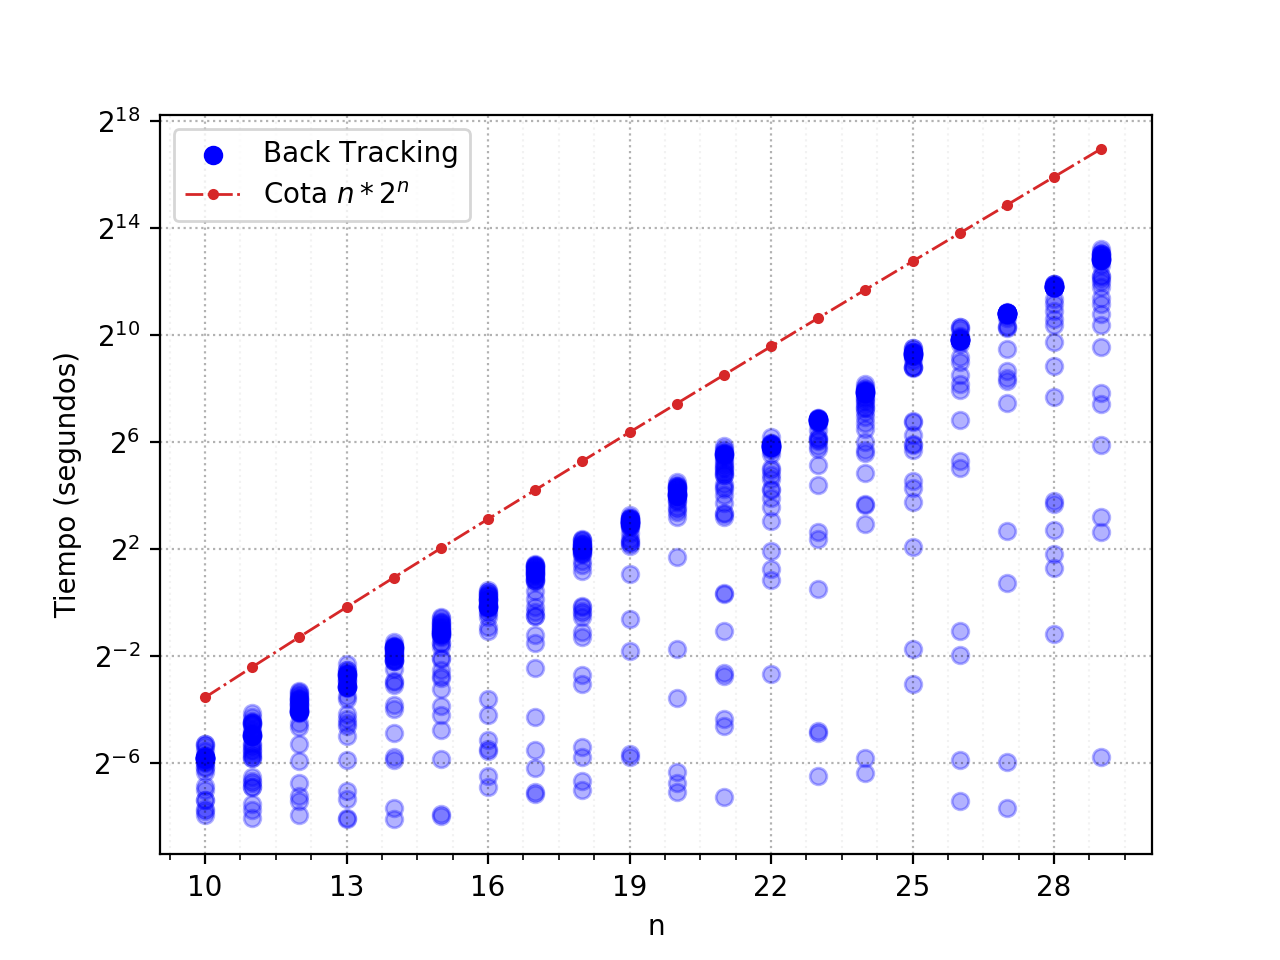
\includegraphics[width=1\textwidth]{bt-and-cota-log}
		\caption{\footnotesize Segundos consumidos (en escala logarítmica) en función de la cantidad de elementos de $values$.}
		\label{fig:plot-bt-and-cota-log}
	\end{minipage}%
\end{figure}

Al igual que en los gráficos de fuerza bruta, la tendencia es clara: la función $f(n)=n*2^n$ acota superiormente al algoritmo de back tracking para todo $n \in \{10, ..., 34\}$. A su vez, queda evidenciado su comportamiento exponencial.

\begin{figure}[H]
	\centering
	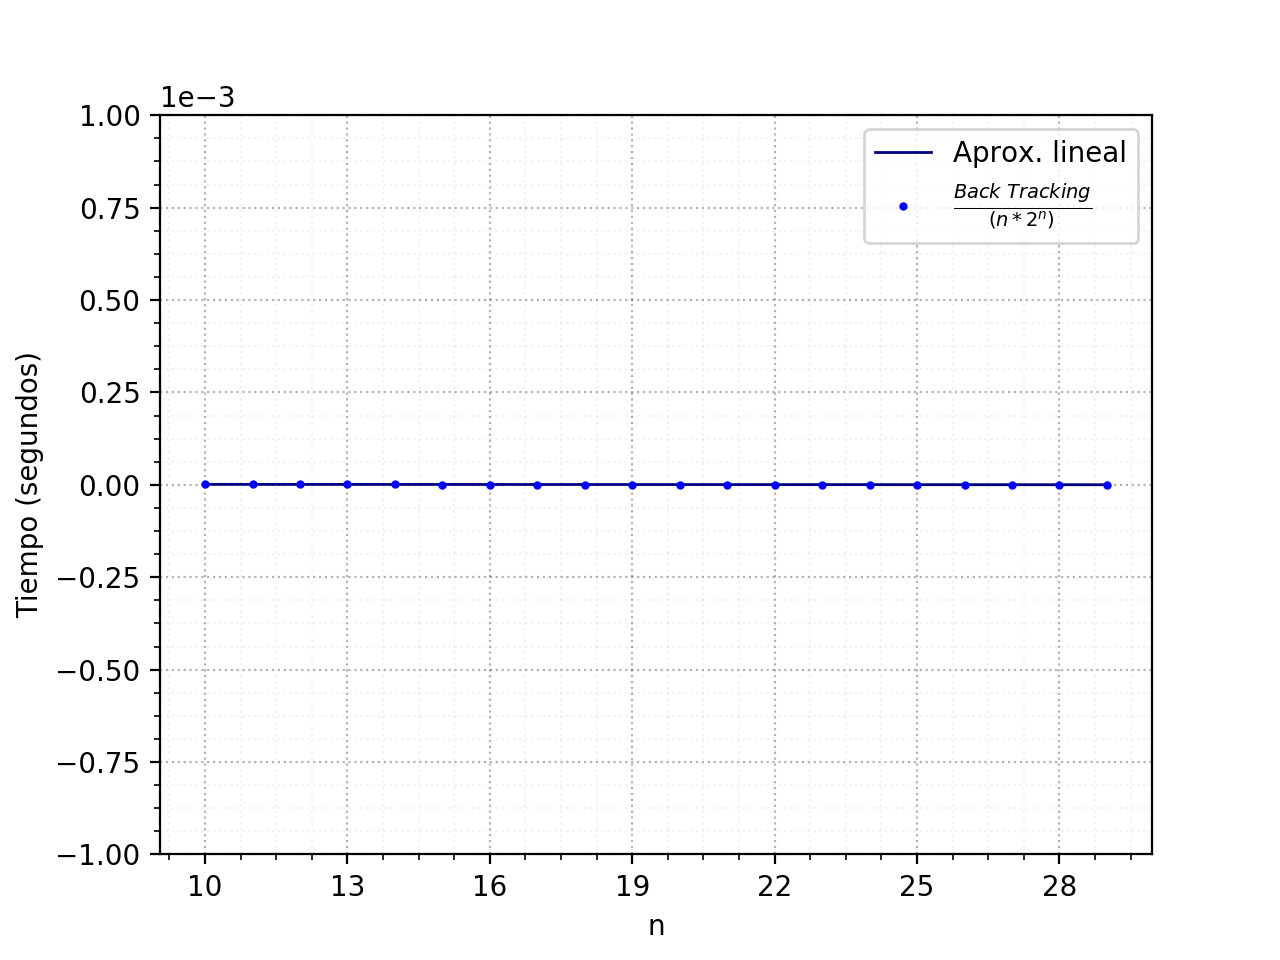
\includegraphics[width=0.5\textwidth]{bt-div-cota}
	\caption{\footnotesize Segundos consumidos en función de la cantidad de elementos de $values$ dividido $n*2^n$}
	\label{fig:plot-bt-div-cota}
\end{figure}

\subsection{Programación Dinámica}
\begin{figure}[H]
	\centering
	\begin{minipage}{0.48\textwidth}
		\centering
		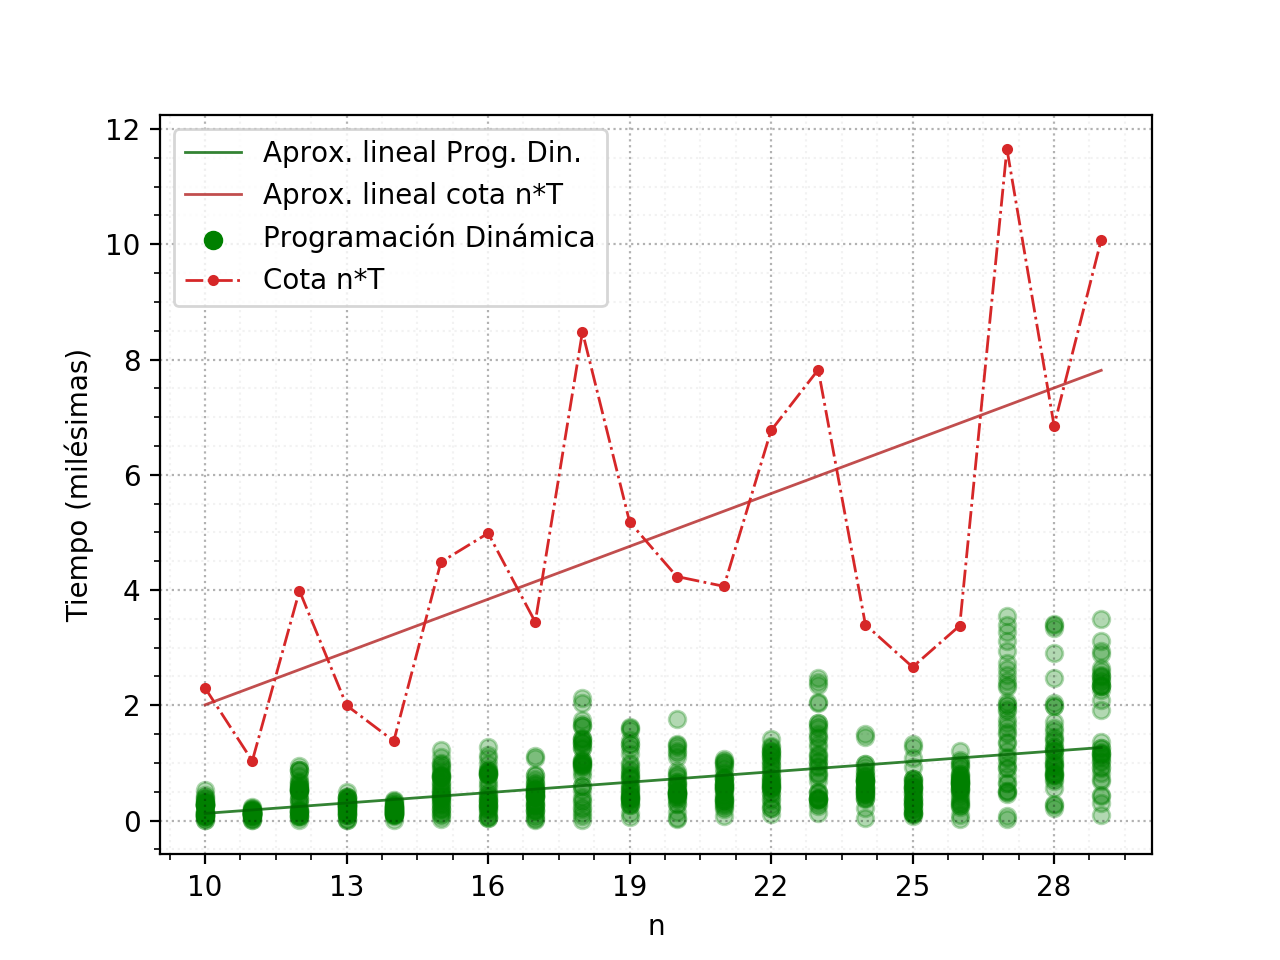
\includegraphics[width=1\textwidth]{pd-and-cota}
		\caption{\footnotesize Segundos consumidos (en escala lineal) en función de la cantidad de elementos de $values$.}
		\label{fig:plot-bf-and-cota}
	\end{minipage}%
	\hspace{0.03\textwidth}
	\begin{minipage}{0.48\textwidth}
		\centering
		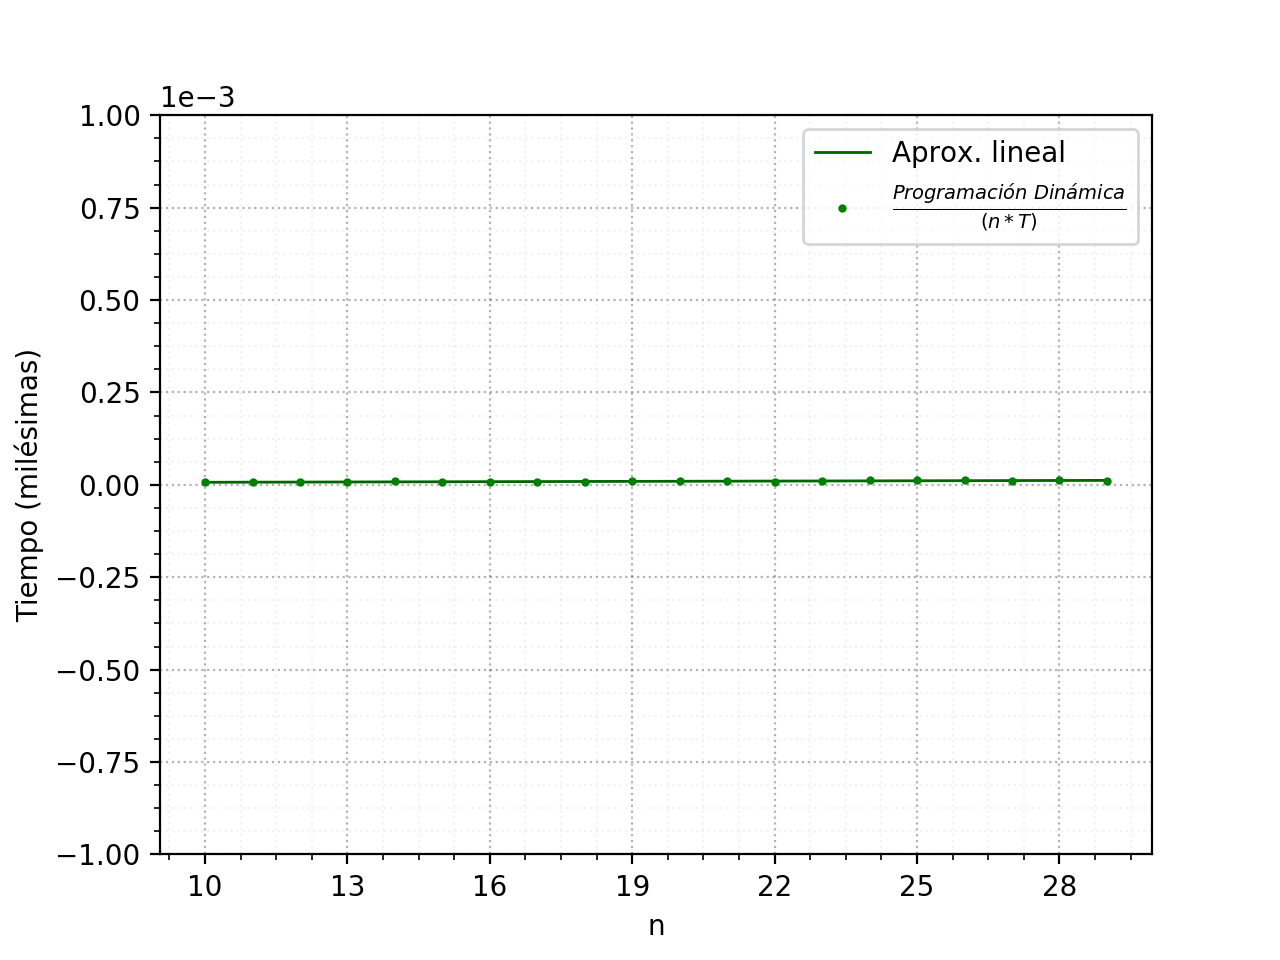
\includegraphics[width=1\textwidth]{pd-div-cota}
		\caption{\footnotesize Segundos consumidos en función de la cantidad de elementos de $values$ dividido $n*T$}
		\label{fig:plot-bf-and-cota-log}
	\end{minipage}%
\end{figure}

En estos experimentos podemos notar una tendencia extraña en el grafico \ref{fig:plot-bf-and-cota}, donde se aprecia una fluctuación alternante en la cota $n*T$. Al evaluar con detenimiento la situación, podemos observar que las depresiones en la cota también se ven reflejadas en las mediciones del algoritmo de programación dinámica. Lo mismo sucede con las elevaciones. Este fenómeno puede ser explicado sencillamente: la cota teórica del algoritmo es $n*T$ que no tiene una traducción directa con los segundos que puede demorar un algoritmo. Para esto, fue necesario calcular la equivalencia en segundos que llamaremos $\delta$ de una operación $\mathcal{O}(1)$ en nuestro algoritmo. Luego, estimamos el costo temporal en segundos de un problema $(V, n, T)$ como $n*T*\delta$. Si bien $\delta$ permanece igual para todos los $n$ (porque se utilizan todos los cardinales para calcularlo), $T$ no permanece inmutable. Es por eso que el valor final de $n*T*\delta$ es afectado por un valor $T$ que es elegido al azar para cada cardinal, explicando el por qué de las depresiones y elevaciones en la cota pero que, a su vez, son respetadas por el algoritmo de programación dinámica.

\subsection{Algoritmo vs algoritmo}
\subsubsection{Entradas densas y aleatorias}
\begin{figure}[H]
	\centering
	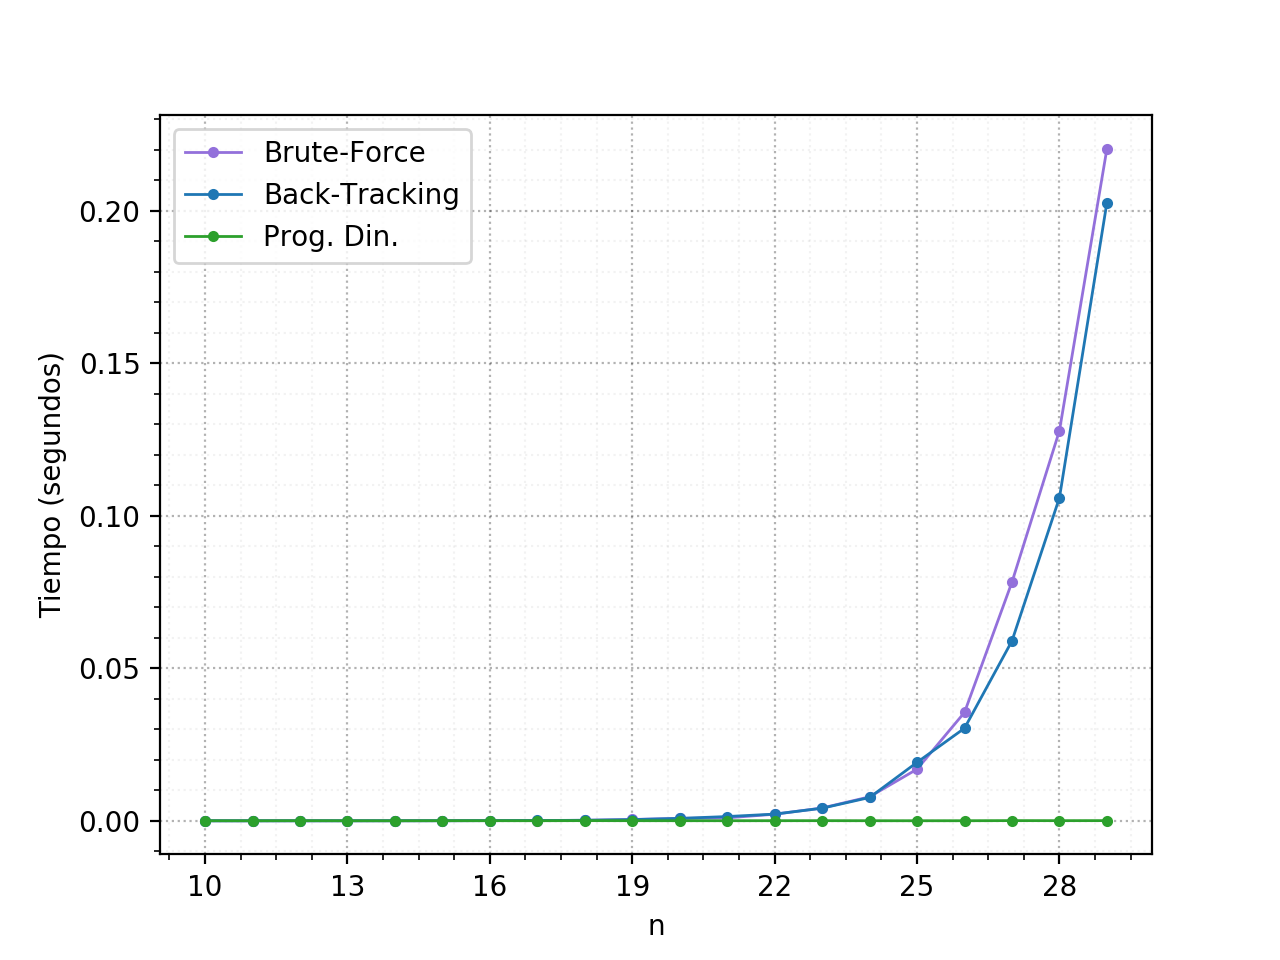
\includegraphics[width=0.5\textwidth]{bf-and-bt-and-pd}
	\caption{\footnotesize Segundos consumidos en función de la cantidad de elementos de $values$}
	\label{fig:bf-and-bt-and-pd}
\end{figure}

Podemos observar la superioridad en performance de la implementación con Programación Dinámica versus Back Tracking y Fuerza Bruta para entradas densas y aleatorias, es decir, con una cantidad alta de elementos. Mientras que la primera es completamente lineal, las dos últimas son exponenciales. Pero este caso se da siempre y cuando la composición de los problemas sea totalmente aleatoria. ¿Qué situación tendríamos si las soluciones se encontrasen en una posición temprana de la lista? ¿Y si el valor objetivo $T$ es muy grande? ¿Y si, en cambio, las listas fuesen pequeñas?

\subsubsection{Soluciones tempranas o tardías con $T$ elevado}
\begin{figure}[H]
	\centering
	\begin{minipage}{0.48\textwidth}
		\centering
		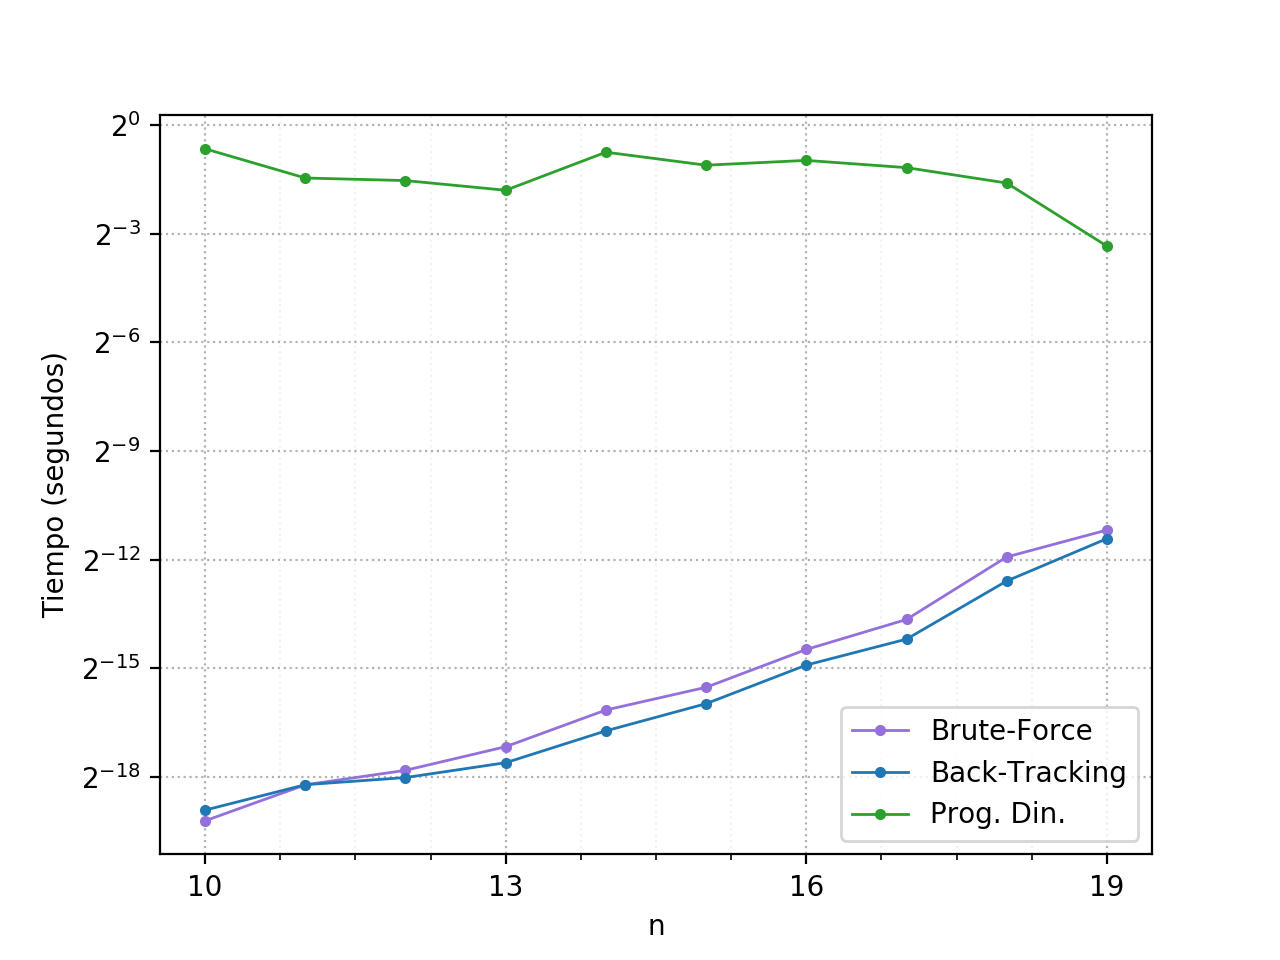
\includegraphics[width=1\textwidth]{bf-and-bt-and-pd-noshuff-nounsolv-head}
		\caption{\footnotesize Problemas sólo con soluciones tempranas (es decir, exclusivamente en el principio de $values$)}
		\label{fig:bf-and-bt-and-pd-noshuff-nounsolv-head}
	\end{minipage}%
	\hspace{0.03\textwidth}
	\begin{minipage}{0.48\textwidth}
		\centering
		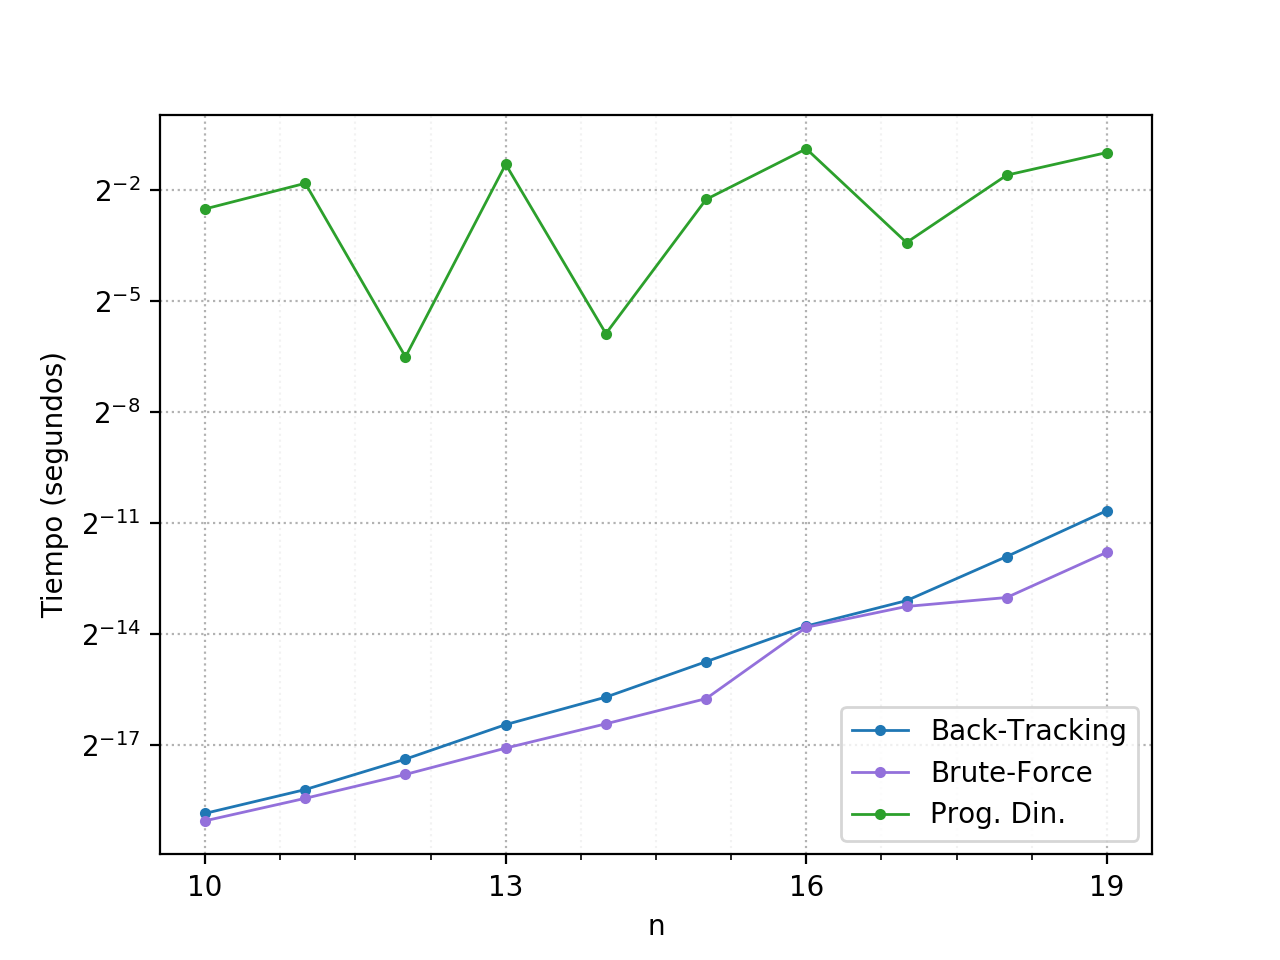
\includegraphics[width=1\textwidth]{bf-and-bt-and-pd-noshuff-nounsolv-tail}
		\caption{\footnotesize Problemas sólo con soluciones tardías (es decir, exclusivamente en el final de $values$)}
		\label{fig:bf-and-bt-and-pd-noshuff-nounsolv-tail}
	\end{minipage}%
\end{figure}

Para este experimento utilizamos un valor $T$ de ocho dígitos decimales. Podemos observar que en ambos casos el algoritmo de Programación Dinámica no tiene un buen desempeño. En cambio, el de Fuerza Bruta y Back Tracking compiten cercanamente. Cuando la solución a los problemas está exactamente al principio de la lista, el algoritmo de fuerza bruta resulta más eficiente y porque este – por como fue implementado – inicia su búsqueda desde el comienzo de la lista. En cambio, cuando la solución está al final de la secuencia, el algoritmo de Back Tracking es ligeramente más rápido por el motivo análogo al anterior: Back Tracking inicia su búsqueda desde el final de la lista de valores. ¿Pero qué pasa con el algoritmo de Programación Dinámica? No parece ser eficiente en ningún aspecto. Hipotetizamos que es por el excesivamente elevado valor de $T$. Analizaremos este aspecto en la siguiente sección.

\subsubsection{Cardinal fijo y valor objetivo dinámico con listas pequeñas}
\begin{figure}[H]
	\centering
	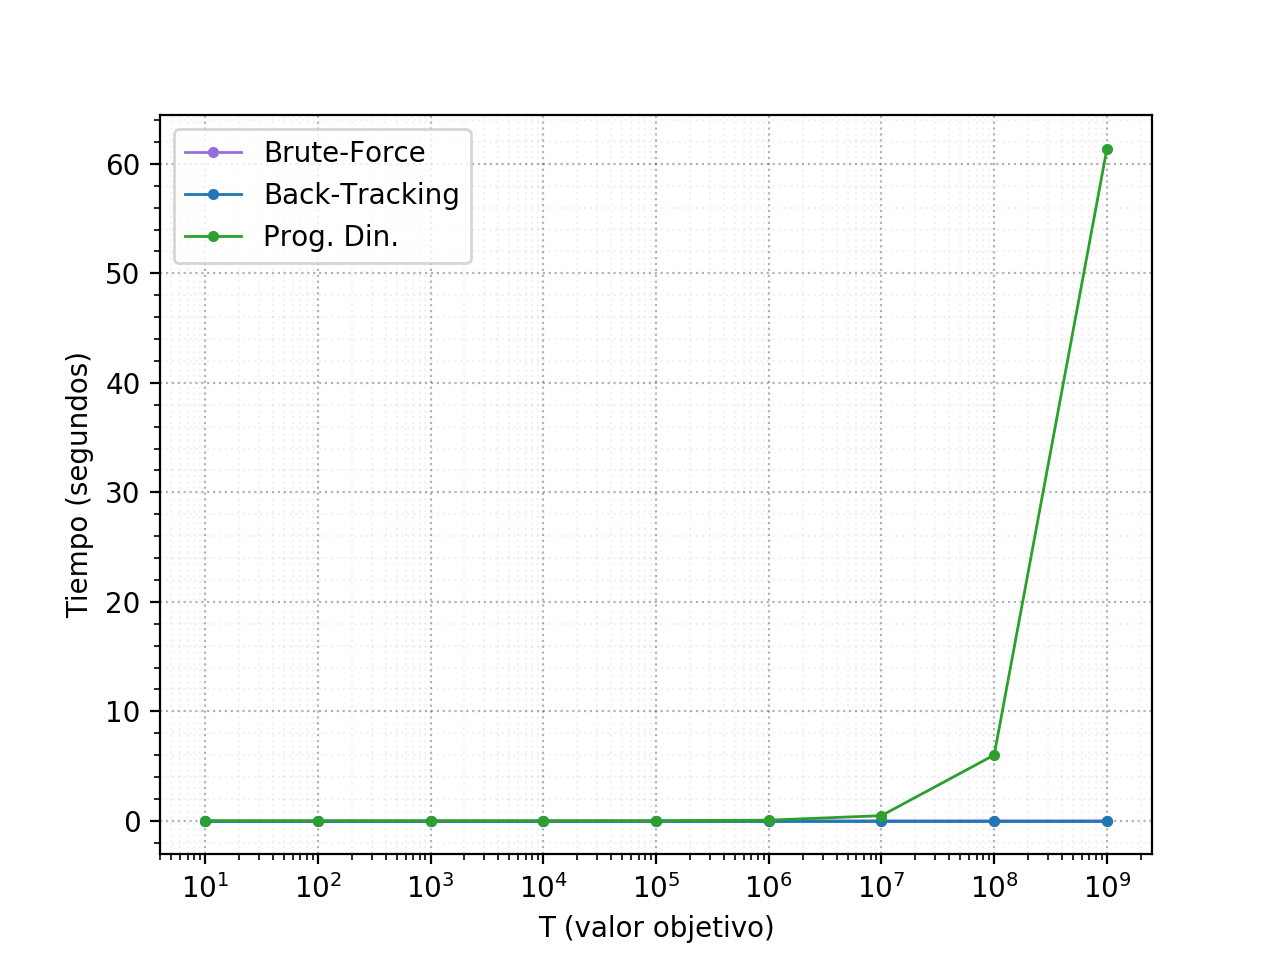
\includegraphics[width=0.5\textwidth]{bf-and-bt-and-pd-shuff-nounsolv-fixed-n}
	\caption{\footnotesize Segundos consumidos en función del valor objetivo T}
	\label{fig:bf-and-bt-and-pd}
\end{figure}
En este experimento fijamos el cardinal de los valores posibles a $n=5$ e iteramos sobre el valor de $T$. Podemos ver que para los algoritmos de Back Tracking y Brute Force, solucionar un problema de tamaño 5 para cualquier $T$ es instantáneo mientras que los tiempos tomados por la implementación de Programación Dinámica aumentan drásticamente a medida que $T$ lo hace.